

\section{MetaPreprocess}

In this section, we introduce how to upload the datasets into the metaOmics software suite,
which is the first step in order to run any of the seven analytical modules.
The R package for MetaPreprocess module can be found at \url{https://github.com/metaOmics/preproc}.

\subsection{Preprocessing page}
\label{sec:procedure}

\begin{steps}
\item \textbf{Uploading data:}

\begin{figure}[!htbp]
\begin{center}
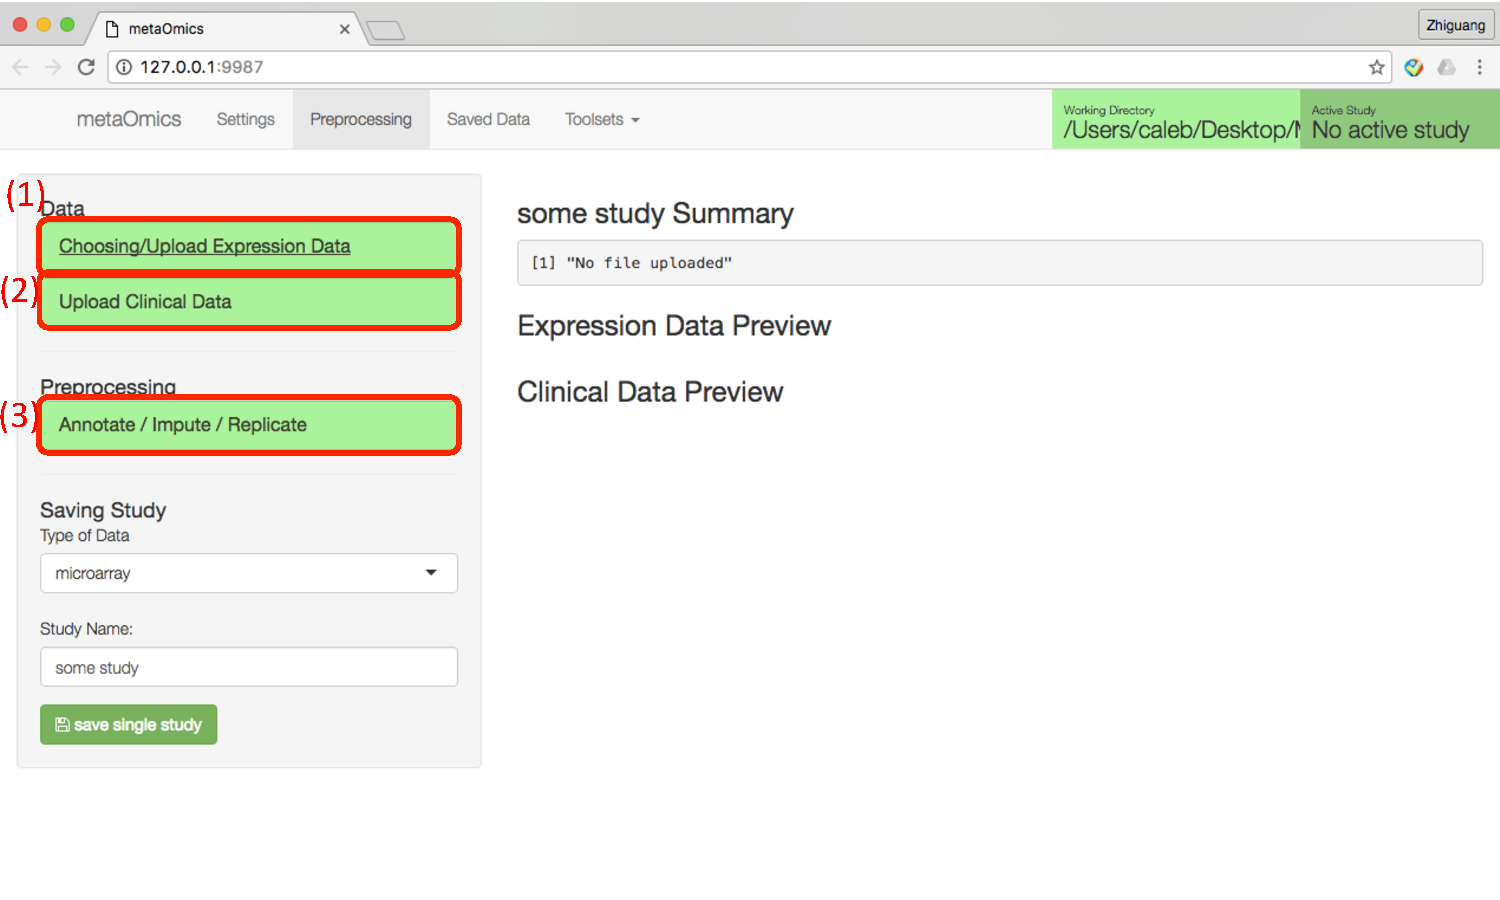
\includegraphics[scale=1]{./figure/preprocessing/GUIpreprocessing}
\caption{GUI Preprocessing page}
\label{fig:GUIpreprocessing}
\end{center}
\end{figure}

In the Preprocessing page,
by clicking on the ``Choosing/Upload Expression Data" tab,
users can upload expression data files (i.e., data file from each study) 
or choose the existing saved data files as in Figure~\ref{fig:GUIpreprocessing} {\color{red} (1)}.
The data should be prepared according to Section~\ref{sec:dataPrepare}.
Users may optionally upload Clinical Data (See Figure~\ref{fig:GUIpreprocessing} {\color{red} (2)}), 
depending on their biological purposes.
Note that all metaOmics modules require external clinical labels except for the MetaClust module.
The three example datasets are available under metaOmics folder ``/metaOmics/data/example/",
and we will mainly focus on the AML dataset (``/metaOmics/data/example/leukemia") throughout this tutorial.
By clicking ``save single study", the gene expression profile will be uploaded and the data can be previewed on the right side of the page.


\item \textbf{Preprocessing:}

The metaOmics software suite also provides handlers (See Figure~\ref{fig:GUIpreprocessing} {\color{red} (3)}) for feature annotation, 
missing value imputation and multiple probes reduction for the same gene.
For preprocessing, 
click on ``Annotate/Impute/Replicate" to 
\begin{enumerate}
\item Annotate the probe ID/reference sequence ID/Entrez ID of individual dataset (choose Gene Symbol if the input data rows are already annotated).
\item Impute missing value using K-Nearest Neighbors (KNN) algorithm.
The algorithm has been described in \cite{troyanskaya2001missing}.
Note that missing value will be automatically detected. 
If there is no missing value, this function will be disabled.

\item Handle the multiple probes matching to the same gene issue.
For the meta-analysis purpose, 
if multiple probes match to the same gene symbol, only one represented gene will be selected.
If each input feature represents a unique gene symbol, this function will be disabled.

\end{enumerate}

A complete introduction of these options is available in Section~\ref{sec:completeList_MetaPreprocess}.
The right side of Figure~\ref{fig:GUIpreview} will show the summary statistics of uploaded data and preview of the data matrix.
There is a search box where users can search for their genes of interest.

\begin{figure}[H]
\begin{center}
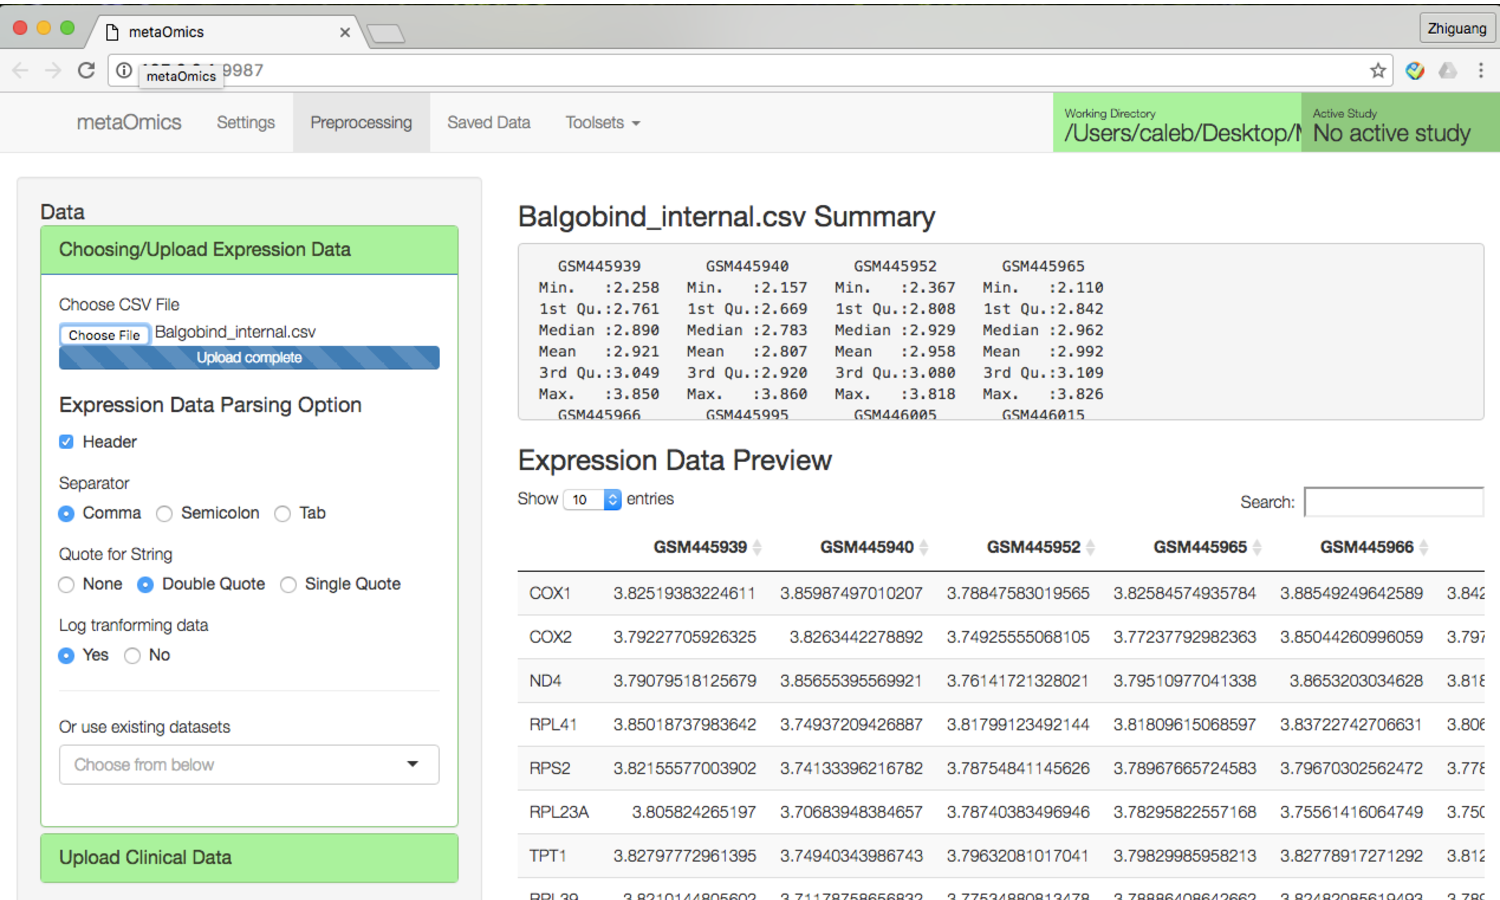
\includegraphics[scale=1]{./figure/preprocessing/GUIpreview}
\caption{Uploading individual studies}
\label{fig:GUIpreview}
\end{center}
\end{figure}

\item \textbf{Save single study:}
In the next step,
specify the data type (microarray data; RNA-seq FPKM/RPKM data; RNA-seq count data) and study name,
and click ``save single study".
To upload RNA-seq data, the count data and FPKM/RPKM
 data should be uploaded separately and saved using different names.
Abbreviation terms for FPKM and RPKM, are explained in Section~\ref{AbbreviationTerms}.

\item \textbf{Upload datasets for all studies:}
Repeat the steps above for all studies in the meta-analysis.
All uploaded studies are now available in the ``Saved Data" page. 
 
\end{steps}

\subsection{Saved Data page}
\label{sec:saved}

After uploading multiple studies w/o clinical data,
users can turn to the Saved Data page.

\begin{figure}[H]
\begin{center}
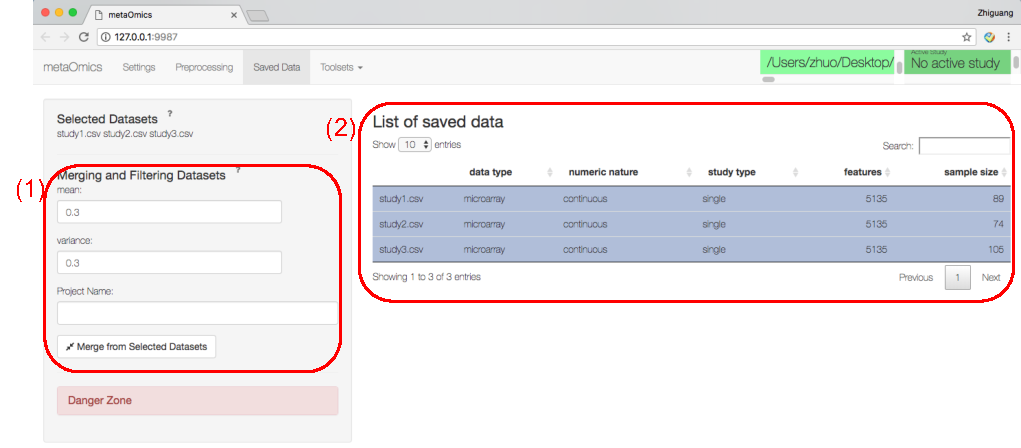
\includegraphics[scale=1]{./figure/preprocessing/GUImerge.pdf}
\caption{Merge from selected datasets}
\label{fig:GUImerge}
\end{center}
\end{figure}


\begin{steps}
\item \textbf{Merging and Filtering:}
All saved datasets from the previous step will be found in  Figure~\ref{fig:GUImerge} {\color{red} (2)}.
Users should select multiple datasets for further meta-analysis.
Users can filter out genes with low expression level (by default, mean expression lower than $30^{th}$ percentile)
or low variance (by default, variance lower than $30^{th}$ percentile).
% a project with stringent filtering criteria keeps  500-1000 genes after the filtering step.
After specifying filtering criteria, enter ``Project Name" and click on the ``Merge from Selected Datasets" (See Figure~\ref{fig:GUImerge} {\color{red} (1)}).
A merged dataset (study type = ``multiple") will appear on the ``List of saved data" panel (Figure~\ref{fig:GUImerge} {\color{red} (2)}).
Creating multiple projects with varying preprocessing criteria is useful.
For example, the user can start from a project with harsh filtering criteria (maintain 500-1000 genes) and give a test run through all modules to save time.
If successful, a larger project can be created by including more genes.
If users want to delete any dataset, they can click on the red ``danger zone" button and delete the selected datasets.

\item \textbf{Make active dataset:}
\label{sec:active}
The last thing to do before using any of the meta-analytic modules is to select the merged data and click on 
``Make your dataset Active Dataset" -- a big green button in Figure~\ref{fig:active}.
Then the merged data will become the active study that shows up on the top right corner of the page.
The active dataset serves as the input for all the analytical modules in metaOmics.

\end{steps}







\begin{figure}[H]
\begin{center}
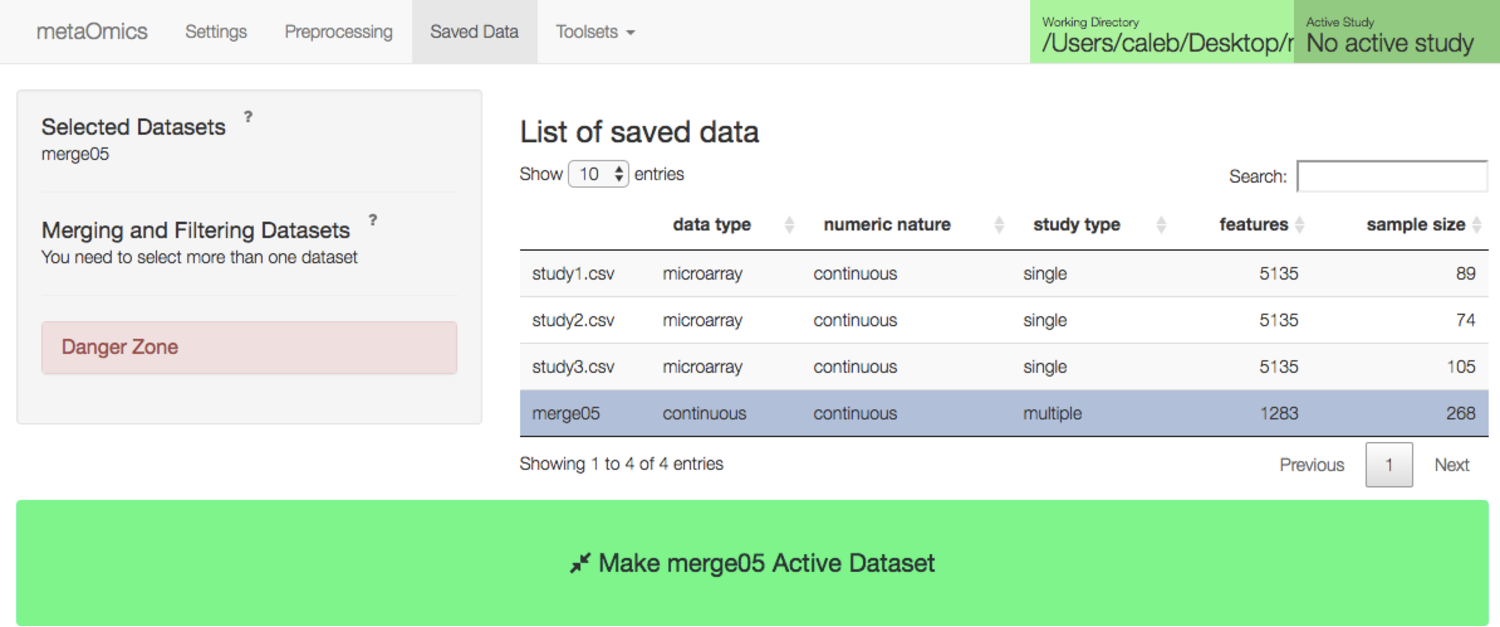
\includegraphics[scale=1]{./figure/preprocessing/GUImarkActive}
\caption{Make merged Dataset Active}
\label{fig:active}
\end{center}
\end{figure}





